\documentclass[14pt, a2paper, landscape]{tikzposter}
\title{Taq DNA Polymerase}
\author{Thomas Holland (th675)}
\usetheme{Simple}

\usepackage{caption}

\usepackage{siunitx}
\usepackage{mhchem}

\usepackage[utf8]{inputenc}
\usepackage[english]{babel}

\usepackage{graphicx}

%\usepackage{biblatex}
%\addbibresource{citations.bib}

\begin{document}
\maketitle
\block{General Info}
{
\textbf{PDB ID:} {1TAQ}
\textbf{Species of origin:} \textit{Thermus aquaticus}
\textbf{Total structure weight:} 94.44 \si{kDa} (\si{\kilo\gram\per\mole})
\textbf{Chain length:} 832 amino acids
\textbf{Atom count:} 6,747 atoms [2]
}

\begin{columns}
    \column{0.5}
    \block{}
    {
    \vspace{-5em}
    \begin{minipage}{.45\linewidth}
    	{\centering
    	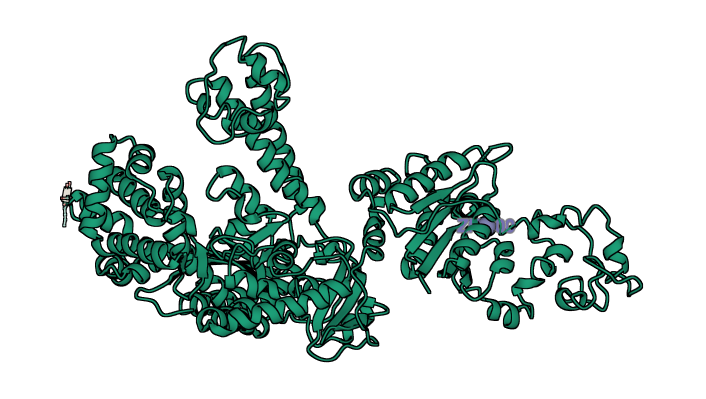
\includegraphics[width=\linewidth]{1TAQ.png}}
    	\captionof{figure}{Taq polymerase with secondary structures, zinc ion, and Carbohydrate group shown. Generated from PDB.}
    \end{minipage}
    \begin{minipage}{.1\linewidth}
    	\ 
    \end{minipage}
    \begin{minipage}{.45\linewidth}
    	{\centering
    	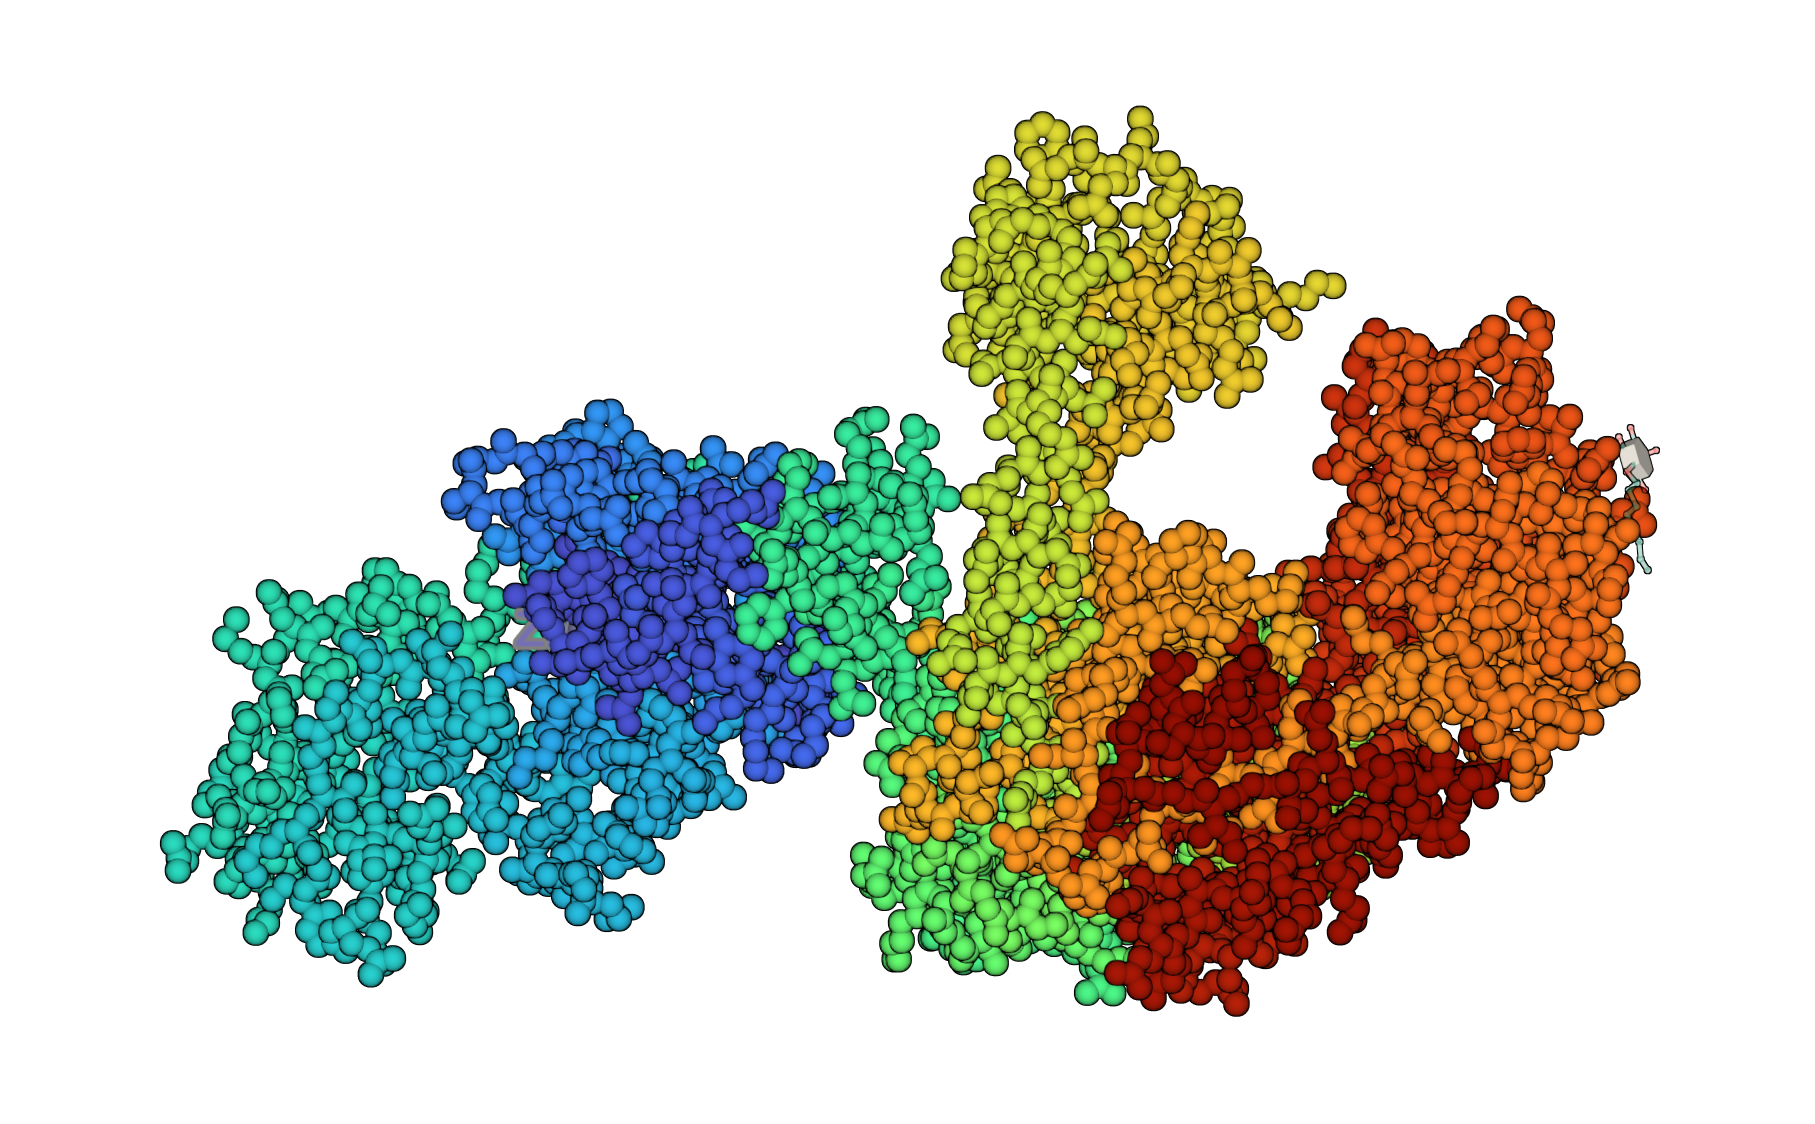
\includegraphics[width=\linewidth]{1TAQ-2.png}}
    	\captionof{figure}{Taq polymerase spatial model with colouring starting at blue from amino terminus to red at carboxyl terminus. Generated from PDB.}
    \end{minipage}
    \vspace{-3em}
    }
    
    \block{Domains}
    {
    The Taq polymerase enzyme has three domain regions, each with a specific role for the function of the enzyme [1]:
    
    	\begin{minipage}{.5\linewidth}
    	\begin{itemize}	
    	\item Amino terminus region: 5' nuclease domain that houses the zinc (\ce{Zn^{2+}}) ion
    	\item Carboxyl terminus region: polymerisation reaction catalyst domain, which is broken into three subdomains:
    	\begin{itemize}
    	\item Palm subdomain
    	\item Fingers subdomain
    	\item Thumb subdomains
    	\end{itemize}
    	\item 3'-5' exonuclease domain located mid-protein
    	\end{itemize}
    	\end{minipage}
    	\hfill
		\begin{minipage}{.5\linewidth}
			\centering
			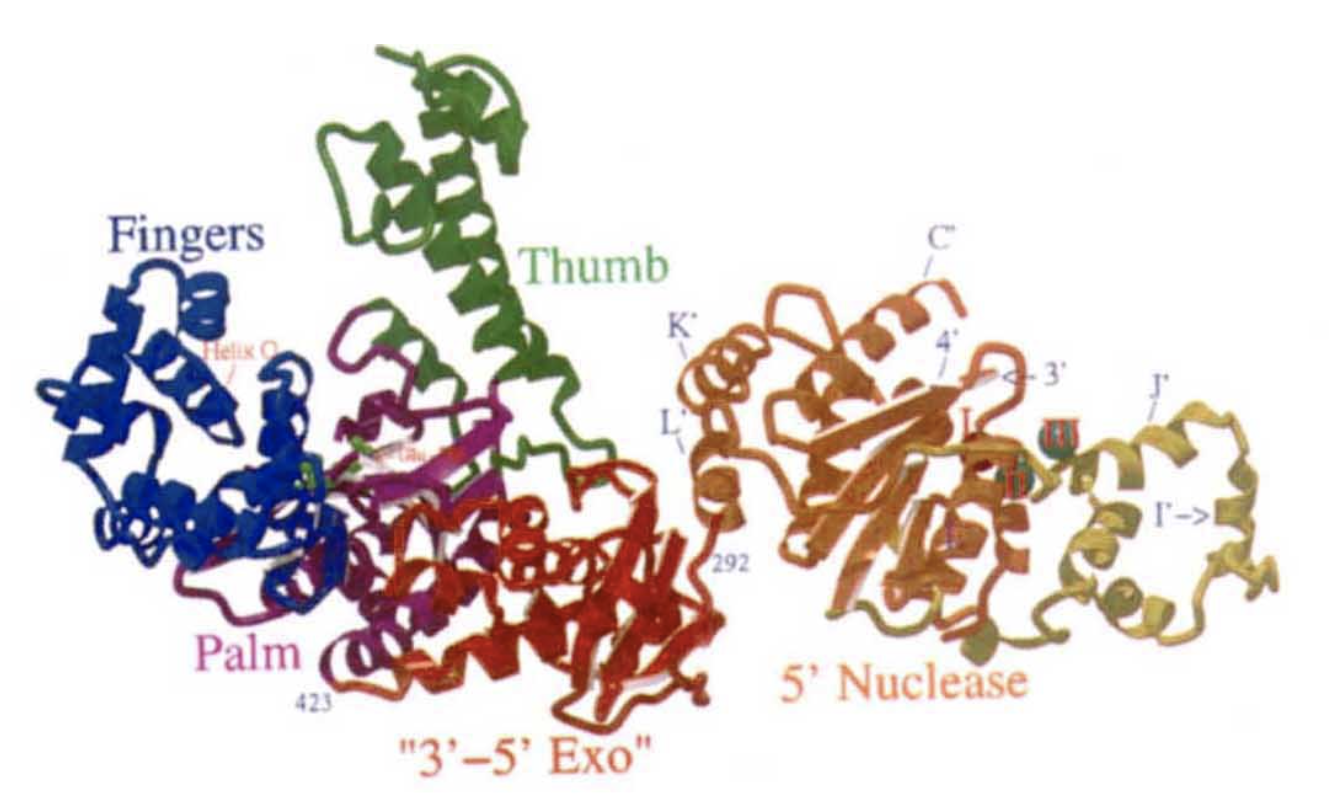
\includegraphics[width=\linewidth]{Screenshot1}
			\captionof{figure}{Taq Polymerase structure, coloured by domain [1]}
		\end{minipage}
	}
    \column{0.5}
   	\block{}{Taq polymerase is a thermostable DNA polymerase that is found within the thermophilic \textit{Thermus aquaticus} bacteria. It was the first thermostable polymerase to be discovered and isolated, and is commonly used for Polymerise Chain Reaction (PCR), in which the enzymes need to withstand high temperatures, to amplify short quantities of DNA for further analysis and other uses.
   	\vspace{-3em}}
    
    \block{Ligands}
    {
    There are two ligands within Taq polymerase:
    
	\begin{minipage}{0.5\linewidth}
    	    \begin{description}
    	\item[Zinc ion (\ce{Zn^{2+}})]
    	\item[2-O-octyl-beta-D-glucopyranose (BGL)]
    	A D-isomer form of the saccharide that has eight sided ring joined to the D-glucopyranos via a beta glycosidic bond.
    \end{description}
    \end{minipage}
    \begin{minipage}{0.5\linewidth}
    \centering
    	    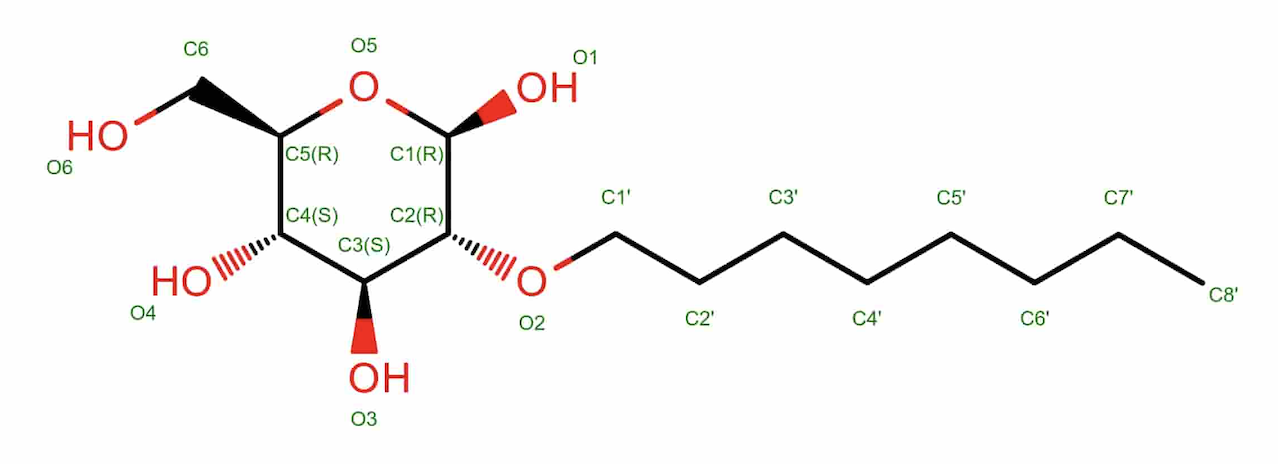
\includegraphics[width=\linewidth]{BGL}
    	    
    	   \captionof{figure}{2-O-octyl-beta-D-glucopyranose (BGL), the carbohydrate ligand within Taq Polymerase [3]}
    \end{minipage}
    \vspace{-5em}
    }
    \block{References}
    {
\begin{definition}
	\item[[1]] Y Kim et al. Crystal structure of Thermus aquaticus DNA polymerase. Nature. 376(6541):612–616, August 1995. doi: 10.1038/376612a0.
	\item[[2]] Protein Data Bank. RCSB PDB - 1TAQ: STRUCTURE OF TAQ DNA POLYMERASE. https://www.rcsb.org/structure/1TAQ. Accessed: 2022-11-02.
	\item[[3]] Protein Data Bank. RCSB PDB - BGL Ligand Summary Page. https://www.rcsb.org/ligand/BGL. Accessed: 2022-b-11-02.
\end{definition}



    }

    
    
   
\end{columns}
%\block{References}{\printbibliography[title={}]}
\end{document}